\def\nomebase{ExamExample1} 
\DTLifdbexists{\nomebase}{}{\DTLloaddb{\nomebase}{ExamExample1.csv}} 
 
\makeatletter 
\@ifundefined{contagem\nomebase}{% 
\def\contagem\nomebase{\DTLrowcount{\nomebase}} 
}{} 
\makeatother 
  
\makeatletter 
\def\numprova{\the\AMCid@etud} 
\makeatother 
  
%####Descomentar linha a seguir para buscar as linhas do csv de forma sequencial, de acordo com o n�mero da prova 
\FPeval\numlinha{round(\numprova-(\contagem\nomebase)*trunc((\numprova-1)/(\contagem\nomebase),0),0)} 
  
%####Descomentar linha a seguir para buscar as linhas no csv de forma aleatoria 
%\FPeval\numlinha{round(1+random*(\contagem\nomebase -1),0)} 
  
\DTLgetvalue{\V}{\nomebase}{\numlinha}{1} 
\DTLgetvalue{\ITwo}{\nomebase}{\numlinha}{2} 
\DTLgetvalue{\IThree}{\nomebase}{\numlinha}{3} 
\DTLgetvalue{\PThree}{\nomebase}{\numlinha}{4} 
  
\DTLgetvalue{\idEnunciadoA}{\nomebase}{\numlinha}{5} 
\DTLgetvalue{\EnunciadoA}{\nomebase}{\numlinha}{6} 
\DTLgetvalue{\RespostaA}{\nomebase}{\numlinha}{7} 
\DTLgetvalue{\DigitsRespostaA}{\nomebase}{\numlinha}{8} 
\DTLgetvalue{\DecimalsRespostaA}{\nomebase}{\numlinha}{9} 
\DTLgetvalue{\FaixaExatoRespostaA}{\nomebase}{\numlinha}{10} 
\DTLgetvalue{\MargemRespostaA}{\nomebase}{\numlinha}{11} 
  
\DTLgetvalue{\idEnunciadoB}{\nomebase}{\numlinha}{12} 
\DTLgetvalue{\EnunciadoB}{\nomebase}{\numlinha}{13} 
\DTLgetvalue{\RespostaB}{\nomebase}{\numlinha}{14} 
\DTLgetvalue{\DigitsRespostaB}{\nomebase}{\numlinha}{15} 
\DTLgetvalue{\DecimalsRespostaB}{\nomebase}{\numlinha}{16} 
\DTLgetvalue{\FaixaExatoRespostaB}{\nomebase}{\numlinha}{17} 
\DTLgetvalue{\MargemRespostaB}{\nomebase}{\numlinha}{18} 
  
\DTLgetvalue{\idEnunciadoC}{\nomebase}{\numlinha}{19} 
\DTLgetvalue{\EnunciadoC}{\nomebase}{\numlinha}{20} 
\DTLgetvalue{\RespostaC}{\nomebase}{\numlinha}{21} 
\DTLgetvalue{\DigitsRespostaC}{\nomebase}{\numlinha}{22} 
\DTLgetvalue{\DecimalsRespostaC}{\nomebase}{\numlinha}{23} 
\DTLgetvalue{\FaixaExatoRespostaC}{\nomebase}{\numlinha}{24} 
\DTLgetvalue{\MargemRespostaC}{\nomebase}{\numlinha}{25} 
  
\ifthenelse{\equal{\EnunciadoA}{vazio}}{}{\FPeval\FaixaExatoA{round(abs(\FaixaExatoRespostaA)*10^\DecimalsRespostaA,0)}} 
\ifthenelse{\equal{\EnunciadoB}{vazio}}{}{\FPeval\FaixaExatoB{round(abs(\FaixaExatoRespostaB)*10^\DecimalsRespostaB,0)}} 
\ifthenelse{\equal{\EnunciadoC}{vazio}}{}{\FPeval\FaixaExatoC{round(abs(\FaixaExatoRespostaC)*10^\DecimalsRespostaC,0)}} 
  
\ifthenelse{\equal{\EnunciadoA}{vazio}}{}{\FPeval\MargemA{round(abs(\MargemRespostaA)*10^\DecimalsRespostaA,0)}} 
\ifthenelse{\equal{\EnunciadoB}{vazio}}{}{\FPeval\MargemB{round(abs(\MargemRespostaB)*10^\DecimalsRespostaB,0)}} 
\ifthenelse{\equal{\EnunciadoC}{vazio}}{}{\FPeval\MargemC{round(abs(\MargemRespostaC)*10^\DecimalsRespostaC,0)}} 
  
In the following circuit, where source voltage is $V_s$ = \V~V, current and active power measurements were taken: 
\begin{itemize} 
\item $I_2$ = \ITwo~A; 
\item $I_3$ = \IThree~A; 
\item $P_3$ = \PThree~W (measured in RL branch) 
\end{itemize} 
  
\begin{figure}[htb!] 
\centering 
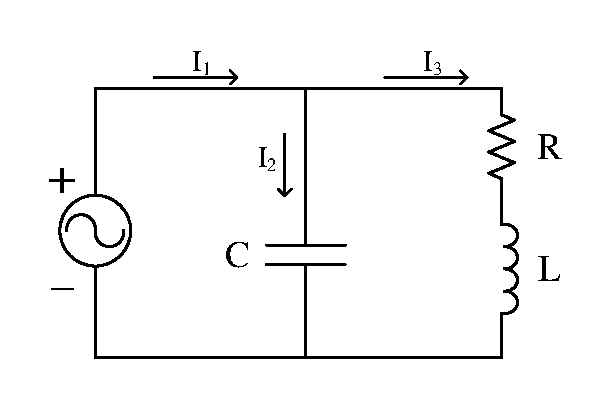
\includegraphics{drawing1.pdf} 
\caption{\footnotesize{Circuit}} 
\label{fig:circuitoExamExample1} 
\end{figure} 
  
\ifthenelse{\equal{\EnunciadoA}{vazio}}{}{ 
\vspace{1cm} 
\begin{questionmultx}{q A\idEnunciadoA} 
\EnunciadoA 
\AMCnumericChoices{\RespostaA{}}{digits=\DigitsRespostaA,decimals=\DecimalsRespostaA,sign=false,borderwidth=1pt,approx=\MargemA,exact=1,vertical=true,hspace=0.3em,vspace=0.5ex,scoreexact=2,scoreapprox=1.5} 
  
\end{questionmultx}} 
  
\ifthenelse{\equal{\EnunciadoB}{vazio}}{}{ 
\vspace{1cm} 
\begin{questionmultx}{q B\idEnunciadoB} 
\EnunciadoB 
\AMCnumericChoices{\RespostaB{}}{digits=\DigitsRespostaB,decimals=\DecimalsRespostaB,sign=false,borderwidth=1pt,approx=\MargemB,exact=1,vertical=true,hspace=0.3em,vspace=0.5ex,scoreexact=2,scoreapprox=1.5} 
  
\end{questionmultx}} 
  
\ifthenelse{\equal{\EnunciadoC}{vazio}}{}{ 
\vspace{1cm} 
\begin{questionmultx}{q C\idEnunciadoC} 
\EnunciadoC 
\AMCnumericChoices{\RespostaC{}}{digits=\DigitsRespostaC,decimals=\DecimalsRespostaC,sign=false,borderwidth=1pt,approx=\MargemC,exact=1,vertical=true,hspace=0.3em,vspace=0.5ex,scoreexact=3,scoreapprox=2} 
  
\end{questionmultx}} 
  
% Open question 
\begin{question}{open-ExamExample1}Describe the procedure and assumptions that should be followed to find the capacitor that adjusts the power factor to a specific value. 
  
~\AMCOpen{lines=5, dots=false, framerule=0pt}{ 
\wrongchoice[\tiny 0]{\tiny 0}\scoring{0}\wrongchoice[\tiny 0.5]{\tiny 0.5}\scoring{0.5}\wrongchoice[\tiny 1]{\tiny 1}\scoring{1}\wrongchoice[\tiny 1.5]{\tiny 1.5}\scoring{1.5}\wrongchoice[\tiny 2]{\tiny 2}\scoring{2}\wrongchoice[\tiny 2.5]{\tiny 2.5}\scoring{2.5}\correctchoice[\tiny 3]{\tiny 3}\scoring{3}} 
\end{question}